%%%%%%%%%%%%%%%%%%%%%%%%%%%%%%%%%%%%%%%%%
% Focus Beamer Presentation
% LaTeX Template
% Version 1.0 (8/8/18)
%
% This template has been downloaded from:
% http://www.LaTeXTemplates.com
%
% Original author:
% Pasquale Africa (https://github.com/elauksap/focus-beamertheme) with modifications by
% Vel (vel@LaTeXTemplates.com)
%
% Template license:
% GNU GPL v3.0 License
%
% Important note:
% The bibliography/references need to be compiled with bibtex.
%
%%%%%%%%%%%%%%%%%%%%%%%%%%%%%%%%%%%%%%%%%

%----------------------------------------------------------------------------------------
%	PACKAGES AND OTHER DOCUMENT CONFIGURATIONS
%----------------------------------------------------------------------------------------

\documentclass{beamer}

\usetheme{focus} % Use the Focus theme supplied with the template
% Add option [numbering=none] to disable the footer progress bar
% Add option [numbering=fullbar] to show the footer progress bar as always full with a slide count

% Uncomment to enable the ice-blue theme
%\definecolor{main}{RGB}{92, 138, 168}
%\definecolor{background}{RGB}{240, 247, 255}

%------------------------------------------------

\usepackage[french]{babel}
\usepackage{booktabs} % Required for better table rules
\usepackage{csquotes}
\usepackage{emoji}
\usepackage{hyperref}
\usepackage{minted}
\usepackage[T1]{fontenc}
\usepackage{xcolor} % to access the named colour LightGray
\definecolor{LightGray}{gray}{0.9}

\hypersetup{
    pdfborderstyle={/S/U/W 1}
}


\AtBeginSection[]
{\begin{frame}
    \frametitle{Sommaire}
    \tableofcontents[currentsection]
\end{frame}
}
%----------------------------------------------------------------------------------------
%	 TITLE SLIDE
%----------------------------------------------------------------------------------------

\title{Les index PostgreSQL}

\subtitle{Et leur intégration avec Django}

\author{\href{mailto:mail@franek.fr}{François FREITAG}}

\titlegraphic{\vspace{30pt} 
\includegraphics[scale=0.15]{Images/elephant.png}}

\institute{Les emplois de l'inclusion \\ GIP Inclusion}

\date{26 août 2024}

%------------------------------------------------

\begin{document}

%------------------------------------------------

\begin{frame}
	\maketitle % Automatically created using the information in the commands above
\end{frame}

%----------------------------------------------------------------------------------------
%	 SECTION 1
%----------------------------------------------------------------------------------------

\section{Le scan séquentiel} % Section title slide, unnumbered

\begin{frame}[fragile]
    \frametitle{Les données, la requête}

    \begin{minted}[bgcolor=LightGray]{sql}
CREATE TABLE test1 (
    id INTEGER,
    content VARCHAR
);
    \end{minted}

    \begin{minted}[bgcolor=LightGray]{sql}
SELECT content FROM test1 WHERE id = constant;
    \end{minted}
\end{frame}

\begin{frame}[fragile]
    \frametitle{EXPLAIN ANALYZE}
    \texttt{ANALYZE} : Carry out the command and show actual run times and other statistics.
    \begin{minted}[bgcolor=LightGray,fontsize=\footnotesize]{sql}
EXPLAIN ANALYZE SELECT content FROM test1 WHERE id = 12;

                     QUERY PLAN
--------------------------------------------------------------
 Seq Scan on test1  (cost=0.00..25.88 rows=6 width=32)
                    (actual time=0.016..0.017 rows=0 loops=1)
   Filter: (id = 12)
 Planning Time: 2.165 ms
 Execution Time: 0.098 ms
(4 rows)
    \end{minted}
\end{frame}

\section{Indexer les données}

\begin{frame}[fragile]
    \frametitle{Indexer les données}
    De la même manière qu'un livre contient souvent un index trié par ordre alphabétique, la base de données crée un index trié des données présentes dans une table.
    \begin{minted}[bgcolor=LightGray,fontsize=\footnotesize]{sql}
CREATE INDEX test1_id_index ON test1 (id);
    \end{minted}
    \vspace{-25pt}
    \begin{minted}[bgcolor=LightGray,fontsize=\footnotesize]{sql}
EXPLAIN ANALYZE SELECT content FROM test1 WHERE id = 12;

                         QUERY PLAN
----------------------------------------------------------------
 Bitmap Heap Scan on test1  (cost=4.20..13.67 rows=6 width=32)
                            (actual time=0.010..0.011 rows=0 loops=1)
   Recheck Cond: (id = 12)
   ->  Bitmap Index Scan on test1_id_index
                (cost=0.00..4.20 rows=6 width=0)
                (actual time=0.008..0.008 rows=0 loops=1)
         Index Cond: (id = 12)
 Planning Time: 0.118 ms
 Execution Time: 0.053 ms
(6 rows)
    \end{minted}
\end{frame}

\begin{frame}{Les coûts d'un index}
    \begin{itemize}
        \item Espace disque supplémentaire
        \item Maintenance de l'index lors des opérations en écriture (\texttt{INSERT}, \texttt{UPDATE}, \texttt{DELETE})
    \end{itemize}
\end{frame}

\section{Les types d'index}

\begin{frame}{B-Tree}
    \begin{itemize}
        \item Index par défaut de PostgreSQL
        \item Equality (\texttt{=}), range queries (\texttt{<}, \texttt{>}, \texttt{BETWEEN}, \texttt{IN}), \texttt{NULL}
    \end{itemize}
    \begin{figure}[b]
        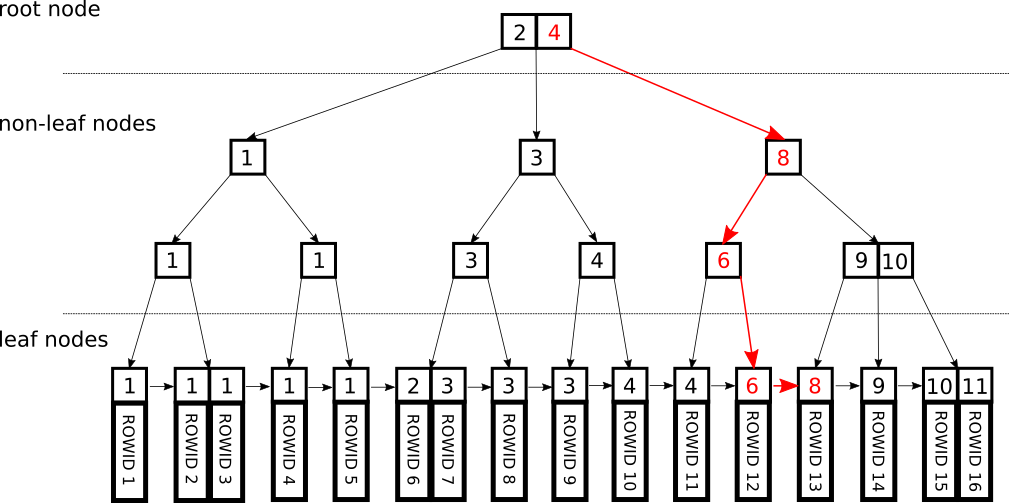
\includegraphics[width=0.9\textwidth]{Images/index_lookup.png}
        \caption{source: \href{https://www.qwertee.io/blog/postgresql-b-tree-index-explained-part-1/}{https://www.qwertee.io/blog/postgresql-b-tree-index-explained-part-1/}}
    \end{figure}
\end{frame}

\begin{frame}{Hash}
    \begin{itemize}
        \item Hash indexes store a 32-bit hash code derived from the value of the indexed column.
        \item Equality (\texttt{=}), not inequality.
        \item More compact and can be faster than a B-Tree index
    \end{itemize}

    \begin{figure}[b]
        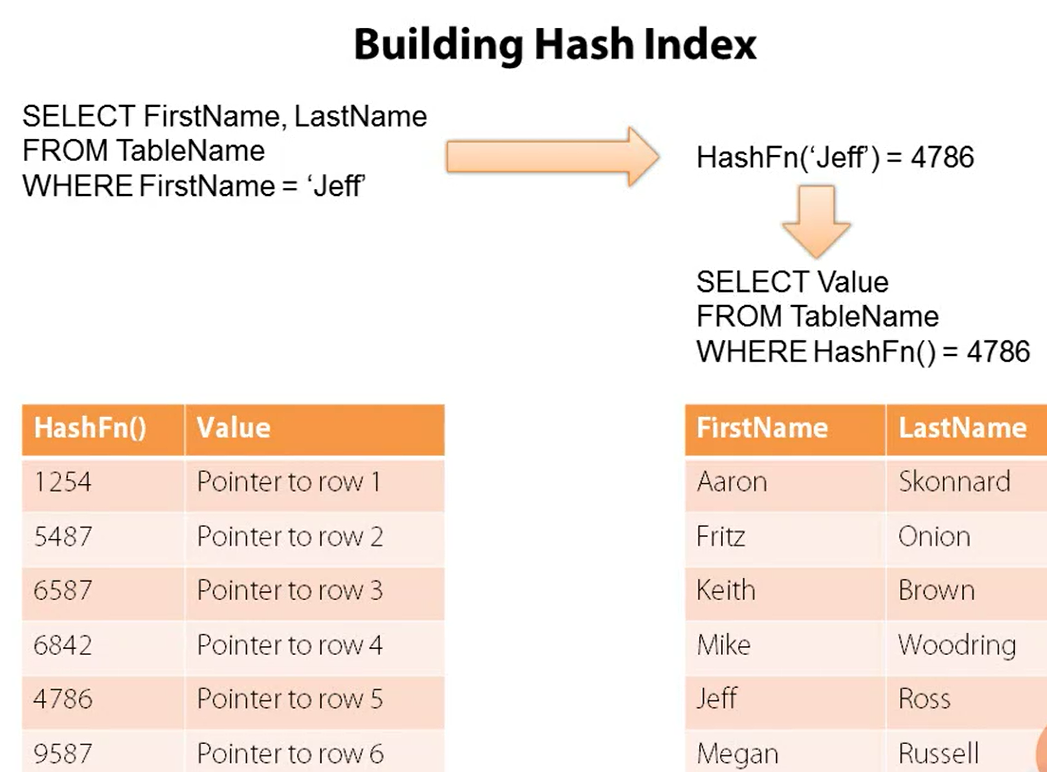
\includegraphics[width=6cm]{Images/hash_index.png}
        \caption{source: \href{https://gss-portal.com/knowledgebase/129/Hash-Index-Part-4.html/}{https://gss-portal.com/knowledgebase/129/Hash-Index-Part-4.html/}}
    \end{figure}
\end{frame}

\begin{frame}{GiST - Generalized Search Tree}
    \begin{itemize}
        \item A balanced, tree-structured access method, that acts as a base template in which to implement arbitrary indexing schemes.
        \item Works on ranges (containment \texttt{<@}, overlap \texttt{\&\&}, strictly left/right \texttt{<<}, \texttt{>>}, etc)
        \item Handles
            \begin{itemize}
                \item ranges (integer, dates, IP subnets, etc),
                \item geographical data,
                \item string distance,
                \item bioinformatics,
                \item nearest neighbors,
                \item and generally what domain experts can modelize with a set of standard operations.
            \end{itemize}
    \end{itemize}
\end{frame}

\begin{frame}{SP-GiST - space-partitioned GiST}
    \begin{itemize}
        \item Same as GiST, but allows for unbalanced structures.
        \item Can be much faster for domains where partitioning makes sense.
    \end{itemize}
\end{frame}

\begin{frame}{GIN - General INverted}
    \begin{itemize}
        \item Appropriate for data values that contain multiple component values, such as arrays or JSON.
        \item Equality (\texttt{=}), containment (\texttt{<@}, \texttt{@>}), overlap (\texttt{\&\&}).
    \end{itemize}

    \Rightarrow \hspace{5pt} C'est ce que les \texttt{emails\_email} utilisent, pour rechercher une adresse email dans la liste des champs \texttt{To}, \texttt{Cc} et \texttt{Bcc}.
\end{frame}

\begin{frame}{BRIN - Block Range Index}
    \begin{itemize}
        \item Designed for handling very large tables in which certain columns have some natural correlation with their physical location within the table.
        \item e.g. storing a store's sale orders might have a date column on which each order was placed
        \item Lossy, must recheck the tuples and discarding those that do not match the query conditions
        \item Very small, avoids scanning large parts of the table
        \end{itemize}
\end{frame}

\begin{frame}{Bloom}
    \begin{itemize}
        \item A Bloom filter is a space-efficient data structure that is used to test whether an element is a member of a set.
        \item Lossy, takes a signature based on the data and returns tuples matching the signature
        \item Many attributes and queries test arbitrary combinations of them
        \item Equality (\texttt{=}), not inequality.
        \item Requires an extension
        \item \href{https://www.postgresql.org/docs/current/bloom.html\#BLOOM-EXAMPLES}{\textit{Example on PostgreSQL documentation}}
    \end{itemize}
\end{frame}

\section{Méthodes d'indexation}

\begin{frame}[fragile]
    \frametitle{Functional index}
    \begin{minted}[bgcolor=LightGray,fontsize=\footnotesize]{sql}
CREATE INDEX test1_upper_content_index ON test1 (UPPER(content));
    \end{minted}
    \vspace{-25pt}
    \begin{minted}[bgcolor=LightGray,fontsize=\footnotesize]{sql}
EXPLAIN ANALYZE SELECT content FROM test1 WHERE UPPER(content)='FOO';

                         QUERY PLAN
--------------------------------------------------------------
 Bitmap Heap Scan on test1  (cost=4.20..13.68 rows=6 width=32)
                            (actual time=0.010..0.011 rows=0 loops=1)
   Recheck Cond: (upper((content)::text) = 'FOO'::text)
   ->  Bitmap Index Scan on test1_upper_content_index
                            (cost=0.00..4.20 rows=6 width=0)
                            (actual time=0.008..0.008 rows=0 loops=1)
         Index Cond: (upper((content)::text) = 'FOO'::text)
 Planning Time: 0.142 ms
 Execution Time: 0.055 ms
    \end{minted}
\end{frame}

\begin{frame}[fragile]
    \frametitle{Functional index}

    \emoji{warning} Requires a functional query.
    \begin{minted}[bgcolor=LightGray,fontsize=\footnotesize]{sql}
EXPLAIN ANALYZE SELECT content FROM test1 WHERE content='FOO';

                       QUERY PLAN
------------------------------------------------------
 Seq Scan on test1  (cost=0.00..25.88 rows=6 width=32)
                    (actual time=0.017..0.018 rows=0 loops=1)
   Filter: ((content)::text = 'FOO'::text)
 Planning Time: 0.865 ms
 Execution Time: 0.105 ms
(4 rows)
    \end{minted}
\end{frame}

\begin{frame}{\texttt{CIEmailField}}
    Module \href{https://devdocs.io/postgresql~15/citext}{\texttt{citext}} pour les adresses e-mail des emplois de l’inclusion.

    \begin{itemize}
        \item Comparaison non sensible à la casse
        \item Pas besoin d’appeler de fonction sur les valeurs
        \item Fonctionne avec \texttt{UNIQUE}
        \item Les emails n’ont pas besoin d’une normalisation de l'unicode, car les emplois ne supportent pas l'\textit{Email Address Internationalization}
    \end{itemize}

    Refs \href{https://github.com/gip-inclusion/les-emplois/commit/c2a250388277f429fdc22b89205ef959681471ad}{ce commit}
\end{frame}

\begin{frame}[fragile]
    \frametitle{Partial index}
    \begin{minted}[bgcolor=LightGray,fontsize=\footnotesize]{sql}
CREATE INDEX test1_large_ids_index ON test1 (id) WHERE id >= 300000;
    \end{minted}
    \vspace{-25pt}
    \begin{minted}[bgcolor=LightGray,fontsize=\footnotesize]{sql}
EXPLAIN ANALYZE SELECT * FROM test1 WHERE id > 30000;

                   QUERY PLAN
----------------------------------------------------------------
 Bitmap Heap Scan on test1  (cost=7.43..22.72 rows=423 width=36)
                            (actual time=0.002..0.003 rows=0 loops=1)
   Recheck Cond: (id > 3000000)
   ->  Bitmap Index Scan on test1_composite_index
                            (cost=0.00..7.32 rows=423 width=0)
                            (actual time=0.001..0.002 rows=0 loops=1)
         Index Cond: (id > 30000)
 Planning Time: 0.047 ms
 Execution Time: 0.016 ms
(6 rows)
    \end{minted}
\end{frame}

\begin{frame}[fragile]
    \frametitle{Composite index}
    \begin{minted}[bgcolor=LightGray,fontsize=\footnotesize]{sql}
CREATE INDEX test1_composite_index ON test1 (id, content);
    \end{minted}

    \begin{minted}[bgcolor=LightGray,fontsize=\footnotesize]{sql}
EXPLAIN ANALYZE SELECT * FROM test1 WHERE id > 30000;

                   QUERY PLAN
----------------------------------------------------------------
 Bitmap Heap Scan on test1  (cost=7.43..22.72 rows=423 width=36)
                            (actual time=0.002..0.003 rows=0 loops=1)
   Recheck Cond: (id > 3000000)
   ->  Bitmap Index Scan on test1_composite_index
                            (cost=0.00..7.32 rows=423 width=0)
                            (actual time=0.001..0.002 rows=0 loops=1)
         Index Cond: (id > 30000)
 Planning Time: 0.047 ms
 Execution Time: 0.016 ms
(6 rows)
    \end{minted}
\end{frame}

\begin{frame}[fragile]
    \frametitle{Most specialized index}
    \begin{minted}[bgcolor=LightGray,fontsize=\footnotesize]{sql}
EXPLAIN ANALYZE SELECT * FROM test1 WHERE id > 300000;

                            QUERY PLAN
----------------------------------------------------------------
 Bitmap Heap Scan on test1  (cost=4.24..19.53 rows=423 width=36)
                            (actual time=0.011..0.012 rows=0 loops=1)
   Recheck Cond: (id > 3000000)
   ->  Bitmap Index Scan on test1_large_ids_index
                            (cost=0.00..4.13 rows=423 width=0)
                            (actual time=0.008..0.008 rows=0 loops=1)
         Index Cond: (id > 3000000)
 Planning Time: 0.178 ms
 Execution Time: 0.047 ms
(6 rows)
    \end{minted}
\end{frame}

\section{Django}

\begin{frame}[fragile]
    \frametitle{Django}

    \begin{minted}[bgcolor=LightGray,fontsize=\footnotesize]{python}
class Index(*expressions, fields=(), name=None, db_tablespace=None,
            opclasses=(), condition=None, include=None)

# Un index fonctionnel ?
    \end{minted}
\end{frame}

\begin{frame}[fragile]
    \frametitle{Django}

    \begin{minted}[bgcolor=LightGray,fontsize=\footnotesize]{python}
class Index(*expressions, fields=(), name=None, db_tablespace=None,
            opclasses=(), condition=None, include=None)

# Un index fonctionnel ?
Index(Lower("title").desc(), name="lower_title_idx")
# Un index composite ?
    \end{minted}
\end{frame}

\begin{frame}[fragile]
    \frametitle{Django}

    \begin{minted}[bgcolor=LightGray,fontsize=\footnotesize]{python}
class Index(*expressions, fields=(), name=None, db_tablespace=None,
            opclasses=(), condition=None, include=None)

# Un index fonctionnel ?
Index(Lower("title").desc(), name="lower_title_idx")
# Un index composite ?
Index("title", "pub_date", name="title_date_idx")
# Un index partiel ?
    \end{minted}
\end{frame}

\begin{frame}[fragile]
    \frametitle{Django}

    \begin{minted}[bgcolor=LightGray,fontsize=\footnotesize]{python}
class Index(*expressions, fields=(), name=None, db_tablespace=None,
            opclasses=(), condition=None, include=None)

# Un index fonctionnel ?
Index(Lower("title").desc(), name="lower_title_idx")
# Un index composite ?
Index("title", "pub_date", name="title_date_idx")
# Un index partiel ?
Index(
      "pub_date",
      condition=Q(pub_date__lt=datetime.date(2020, 1, 1)),
      name="published_before_2020_idx",
)
    \end{minted}
\end{frame}

\begin{frame}[fragile]
    \frametitle{Django}

    \begin{minted}[bgcolor=LightGray,fontsize=\footnotesize]{python}
# django.contrib.postgres.indexes:
class BloomIndex(*expressions, length=None, columns=(), **opts): ...
class BrinIndex(*expressions, autosummarize=None,
                pages_per_range=None, **opts): ...
class BTreeIndex(*expressions, fillfactor=None, **opts): ...
class GinIndex(*expressions, fastupdate=None,
               gin_pending_list_limit=None, **opts): ...
class GistIndex(*expressions, buffering=None,
                fillfactor=None, **opts): ...
class HashIndex(*expressions, fillfactor=None, **opts): ...
class SpGistIndex(*expressions, fillfactor=None, **opts): ...
    \end{minted}
\end{frame}

\begin{frame}[focus]
    Merci de votre attention
    \\
    \vspace{20pt}
    \rule{\textwidth}{1pt}
    \\
    \vspace{30pt}
    Avez-vous des questions ?
\end{frame}

\end{document}
